\documentclass[a4paper,11pt,UTF8]{article}
\usepackage{ctex}
\usepackage{amsmath,amsthm,amssymb,amsfonts}
\usepackage{amsmath}
\usepackage[a4paper]{geometry}
\usepackage{graphicx}
\usepackage{microtype}
\usepackage{siunitx}
\usepackage{booktabs}
\usepackage[colorlinks=false, pdfborder={0 0 0}]{hyperref}
\usepackage{cleveref}
\usepackage{esint} 
\usepackage{graphicx}
\usepackage{ragged2e}
\usepackage{pifont}
\usepackage{draftwatermark}
\usepackage{extarrows}
\SetWatermarkLightness{0.97} 
\SetWatermarkText{学数华科}
\title{启明选拔考试数学部分历年题合集}
\author{}
\begin{document}
\maketitle
\noindent
写在开头:

整理了一下历年的启明考试真题以供参考,想通过启明考试转专业的同学可以仔细看看,具体的备考策略可参见转专业群群文件《转专业-数学(时间匆忙 先写一点)》,祝各位考试顺利!
\section*{2023年启明考试数学部分}
\noindent
一.填空题(每题9分)\\
1.若 $\alpha, \beta$ 为正整数且 $\alpha^2+\beta^2=3025$ 则 $\alpha+\beta=$\\
注意到$3025=55^2=(5\times11)^2$,由勾股定理显然可知一种情况$\alpha=3\times11,\beta=4\times11$,\\
故$\alpha+\beta=77$.\\
2. $\displaystyle f(x)+f\left(\frac{1}{\sqrt[3]{1-x^3}}\right)=x^3$. 则 $f(-1)=$\\
注意到$\begin{cases}
	\displaystyle f(-1)+f(\frac{1}{\sqrt[3]{2}})=-1\quad(1)\\
	\displaystyle f(\frac{1}{\sqrt[3]{2}})+f(\sqrt[3]{2})=\frac{1}{2}\quad(2)\\
	\displaystyle f(\sqrt[3]{2})f(-1)=2\quad(3)
\end{cases}$
$\displaystyle(1)+(3)-(2)\Rightarrow f(-1)=\frac{1}{4}$\\
3. $\displaystyle \lim _{n \rightarrow+\infty} \sin ^2\sqrt{n^2+n}\pi$ 的值为\\
$\displaystyle\sin ^2\sqrt{n^2+n} \pi=\sin ^2(\sqrt{n^2+n}-n)\pi=\sin ^2\frac{n}{\sqrt{n^2+n}+n}\pi\\
=\sin ^2\frac{1}{\sqrt{1+\frac{1}{n}}+1}\pi\rightarrow\sin\frac{\pi}{2}=1(n\to\infty)$\\
4. $\beta$ 为锐角. 则 $\displaystyle\left(1+\frac{1}{\sin \beta}\right)\left(1+\frac{1}{\cos \beta}\right)$ 最小值为\\
$\displaystyle(1+\frac{1}{\sin \beta}(1+\frac{1}{\cos \beta})=\frac{\sin\beta\cos\beta+\sin\beta+\cos\beta+1}{\sin\beta\cos\beta}=\frac{\sin\beta+\cos\beta+1}{\sin\beta\cos\beta}+1$\\
令 $\displaystyle t=\sin\beta+\cos\beta=\sqrt{2}\sin(\beta+\frac{\pi}{4})\in(1,\sqrt{2}]$,则$\displaystyle\sin\beta\cos\beta=\frac{t^2-1}{2}$\\
原式$\displaystyle=1+\frac{1+t}{\displaystyle\frac{t^2-1}{2}}=1+\frac{2}{t-1}\geq1+\frac{2}{\sqrt{2}-1}= 3+2\sqrt{2},\beta=\frac{\pi}{4}$取等号.\\
5. $\displaystyle\frac{x^2}{m}+\frac{y^2}{p}=1$ 与$ \displaystyle\frac{x^2}{n}-\frac{y^2}{p}=1(m, n, p>0)$ 有公共焦点 $F_1, F_2$共交点为$Q$.则$S_{\triangle Q F_1 F_2}=\\$
由题意得 $m-n=2 p$,  $m+n=2(m-p)$.\\
$\displaystyle\left\{\begin{array}{l}\displaystyle\frac{x^2}{m}+\frac{y^2}{p}=1, \\ \displaystyle\frac{x^2}{n}-\frac{y^2}{p}=1,\end{array}\right.\Rightarrow x^2=\frac{2 m n}{m+n}, y= \pm \frac{\sqrt{2} p}{\sqrt{m+n}}$\\
$\because\displaystyle\left|F_1 F_2\right|=2 \sqrt{m-p}=2 \sqrt{n+p}$,\\
$\therefore\displaystyle S_{\triangle Q F_1 F_2}=\frac{1}{2} \times 2 \sqrt{m-p} \times \frac{\sqrt{2} p}{\sqrt{m+n}}=p$.\\
6.设 $\varepsilon$ 为1的 7 次方根 $\displaystyle\frac{\varepsilon}{1+\varepsilon^2}+\frac{\varepsilon^2}{1+\varepsilon^4}+\frac{\varepsilon^3}{1+\varepsilon^6}=$\\
对于方程$x^7=1\Rightarrow (x-1)(x^6+x^5+x^4+x^3+x^2+x+1)=0,\varepsilon$为其一个根\\
$\varepsilon=1$,易得原式=$\displaystyle\frac{3}{2}$\\
$\varepsilon\neq1\Rightarrow \varepsilon^6+\varepsilon^5+\varepsilon^4+\varepsilon^3+\varepsilon^2+\varepsilon+1=0$\\
$\displaystyle\frac{\varepsilon}{1+\varepsilon^2}+\frac{\varepsilon^2}{1+\varepsilon^4}+\frac{\varepsilon^3}{1+\varepsilon^6}=\displaystyle\frac{\varepsilon}{1+\varepsilon^2}+\frac{\varepsilon^5}{1+\varepsilon^3}+\frac{\varepsilon^4}{1+\varepsilon}=2\frac{\varepsilon^6+\varepsilon^4+\varepsilon}{(1+\varepsilon^2)(1+\varepsilon^3)}\\
=-2\frac{\varepsilon^5+\varepsilon^3+\varepsilon^2+\varepsilon+1}{(1+\varepsilon^2)(1+\varepsilon^3)}=-2\frac{(1+\varepsilon^2)(1+\varepsilon^3)}{(1+\varepsilon^2)(1+\varepsilon^3)}=-2$\\
7. 三棱柱侧棱垂直底面且所有棱长为$\beta$,则外接球表面积为\\
这道题很简单,画个图很容易得到:$\displaystyle R^2=(\frac{\sqrt{3}}{3}\beta)^2+(\frac{1}{2}\beta)^2\Rightarrow R=\frac{\sqrt{21}}{6}\beta$\\
故$\displaystyle S=4\pi R^2=\frac{7}{3}\pi\beta^2$\\
8.甲组5名男同学、3名女同学,乙组6名男同学、2名女同学,从甲、乙两组各选2
名, 则4人中恰好有一女的选法有\\
分两种情况:\\
case 1: 这名女生来自甲组,共$C_3^1C_5^1C_6^2=225$种\\
case 2: 这名女生来自乙组,共$C_2^1C_6^1C_5^2=120$种\\
故总的选法有345种\\
二.解答题(本题12分)\\
设数列 $\displaystyle\left\{\beta_n\right\}$ 满足 $\displaystyle\beta_1=2 ,\quad \beta_{n+1}-\beta_n=3\times 2^{n-1}$ 记 $\alpha_n=n \beta_n$ 求 $\{\alpha_n\}$ 前 $n$ 项和 \\
$\displaystyle\beta_n=\sum_{k=1}^{n-1}(\beta_{k+1}-\beta_{k})+\beta_1=3\cdot2^{n-1}-1\Rightarrow\alpha_n=3n\cdot2^{n-1}-n$\\
由错位相减法易求得$\displaystyle T_n=\sum_{k=1}^{n}\alpha_k=3(n-1)2^{n}-\frac{n(n+1)}{2}+3$\\
三.解答题(本题16分)\\
已知 $\displaystyle f(x)=\ln (x+1)+\frac{\beta}{x+2}$\\
(i)若 $x>0 , f(x)>1$ 恒成立,求$\beta$取值范围.(6分)\\
$\displaystyle \ln (x+1)+\frac{\beta}{x+2}>1\Rightarrow \beta>(x+2)[1-\ln(x+1)]$\\ 
令$h(x)=(x+2)[1-\ln(x+1), x\in(0,+\infty)$\\
$\displaystyle h^{\prime}(x)=-[\ln(x+1)+\frac{1}{x+1}]<0\Rightarrow h(x)$在$(0,+\infty)$上单调减\\
故$\beta\geq h(0)=2$\\
(ii) 求证 $\displaystyle\ln (2024)>\frac{1}{3}+\frac{1}{5}+\frac{1}{7}+\cdots+\frac{1}{4045}+\frac{1}{4047}$.(10分)\\
由(i)知:$\displaystyle\ln(x+1)>1-\frac{2}{x+2}=\frac{x}{x+2},x>0$\\
取$\displaystyle x=\frac{1}{k}$得到 $\displaystyle\ln(\frac{k+1}{k})>\frac{\displaystyle\frac{1}{k}}{\displaystyle\frac{1}{k}+2}=\frac{1}{2k+1},x>0$\\
故$\displaystyle\ln(2024)=\sum_{k=1}^{2023}\ln(\frac{k+1}{k})>\sum_{k=1}^{2023}\frac{1}{2k+1}$\\
\section*{2022年启明考试数学部分}
\noindent
一.填空题(每题9分)\\
1.已知 $\displaystyle\beta=\frac{\sqrt{5}+1}{2}$, 计算 $\left[\beta^{12}\right]([x]$为$x$的整数部分 $)$.\\
解: $\displaystyle\beta=\frac{\sqrt{5}+1}{2}$ 是方程 $x^2-x-1=0$ 的根, 故: $x^2=x+1, x^4=(x+1)^2=x^2+2 x+1=3 x+2$, $x^{12}=(3 x+2)^3=27 x^3+54 x^2+36 x+8=27 x(x+1)+54(x+1)+36 x+8=27 x^2+117 x+62$ $=27(x+1)+117 x+62=144 x+89 \Rightarrow \beta^{12}=72 \sqrt{5}+161 \in(321,322)$, 故: $\left[\beta^{12}\right]=321$.\\
注释: 考察对偶结构 $\displaystyle\left(\frac{\sqrt{5}+1}{2}\right)^n-\left(\frac{1-\sqrt{5}}{2}\right)^n$ 也是一个重要思想,\\
分析: 熟知Fibonacci $i$ 数列通项: $\displaystyle a_n=\frac{1}{\sqrt{5}}\left[\left(\frac{\sqrt{5}+1}{2}\right)^n-\left(\frac{1-\sqrt{5}}{2}\right)^n\right]$,\\
$\displaystyle\left(\begin{array}{l}\displaystyle a_{n+2}=a_{n+1}+a_n, a_1=a_2=1 \text {, 则特征方程: } x^2=x+1, x_1=\frac{\sqrt{5}+1}{2}, x_2=\frac{1-\sqrt{5}}{2}, \\ \text { 则 }: \displaystyle a_n=C_1\left(\frac{\sqrt{5}+1}{2}\right)^n+C_2\left(\frac{1-\sqrt{5}}{2}\right)^n,\\
\text { 代入初值条件得: } \displaystyle a_n=\frac{1}{\sqrt{5}}\left[\left(\frac{\sqrt{5}+1}{2}\right)^n-\left(\frac{1-\sqrt{5}}{2}\right)^n\right]\end{array}\right)$,\\
解: 令 $\displaystyle a_n=\frac{1}{\sqrt{5}}\left[\left(\frac{\sqrt{5}+1}{2}\right)^n-\left(\frac{1-\sqrt{5}}{2}\right)^n\right]$, 则:\\ $\displaystyle a_{12}=144=\frac{1}{\sqrt{5}}\left[\left(\frac{\sqrt{5}+1}{2}\right)^{12}-\left(\frac{1-\sqrt{5}}{2}\right)^{12}\right]$,
$\displaystyle\left(\frac{\sqrt{5}+1}{2}\right)^{12}=144 \sqrt{5}+\left(\frac{1-\sqrt{5}}{2}\right)^{12}$, 注意到: $144 \sqrt{5}=\sqrt{103680} \in(321.5,322)$,
$\left(\frac{1-\sqrt{5}}{2}\right)^{12} \approx(0.618)^{12} \approx \frac{1}{2^{12}}$, 故: $\left[\beta^{12}\right]=321 . $\\
2.已知: $\beta_1=3, \beta_{n+1}=\beta_n^2-3 \beta_n+4$, 计算: $\displaystyle\sum_{i=1}^{\infty} \frac{1}{\beta_i-1}$\\
解: $\beta_{n+1}=\beta_n^2-3 \beta_n+4 \Rightarrow \beta_{n+1}-2=\beta_n^2-3 \beta_n+2=\left(\beta_n-2\right)\left(\beta_n-1\right)$,\\
则: $\displaystyle\frac{1}{\beta_{n+1}-2}=\frac{1}{\left(\beta_n-2\right)\left(\beta_n-1\right)}=\frac{1}{\beta_n-2}-\frac{1}{\beta_n-1}$, 即: $\displaystyle\frac{1}{\beta_n-1}=\frac{1}{\beta_n-2}-\frac{1}{\beta_{n+1}-2}$, $\displaystyle\sum_{i=1}^{\infty} \frac{1}{\beta_i-1}=1-\lim _{n \rightarrow \infty} \frac{1}{\beta_{n+1}-2}$,\\
下证: $\beta_n$ 单调递增趋于 $+\infty$, 注意到: $\beta_{n+1}-\beta_n=\beta_n^2-4 \beta_n+4=\left(\beta_n-2\right)^2>0$, $\displaystyle\Rightarrow\beta_{n+1}-\beta_1=\sum_{i=1}^n(\beta_i-2)^2>\sum_{i=1}^n(\beta_1-2)^2=n$,故: $\displaystyle\lim _{n \rightarrow \infty} \beta_n=+\infty$, 即: $\displaystyle\sum_{i=1}^{\infty} \frac{1}{\beta_i-1}=1$ .\\
3.已知: $a^2+b^2=5$, 求 $2 a+3 b$ 的最大值,\\
解:\\
Solution 1: $2 a+3 b \leq \sqrt{2^2+3^2} \cdot \sqrt{a^2+b^2}( cauchy )=\sqrt{65}$\\
Solution 2: $2 a+3 b = 2\sqrt{5}\cos\theta+3\sqrt{5}\sin\theta\leq\sqrt{65}$. \\
4.已知: $\left\{\begin{array}{l}x+\sin x \cos x-1=0 \\ 2 \cos y-2 y+\pi+4=0\end{array}\right.$, 求 $\sin (2 x-y)$.\\
解: $\left\{\begin{array}{l}x+\sin x \cos x-1=0 \\ 2 \cos y-2 y+\pi+4=0\end{array} \displaystyle\Rightarrow \left\{\begin{array}{l}2x+ \sin 2 x-2=0\\\displaystyle y-\cos y-\frac{\pi}{2}-2=0\end{array}\right.\right.\displaystyle\Rightarrow \left\{\begin{array}{l}2x+ \sin 2 x-2=0\\\displaystyle y-\frac{\pi}{2}+\sin (y-\frac{\pi}{2})-2=0\end{array}\right.$,\\
观察上式易得同构:  $\displaystyle2 x=y-\frac{\pi}{2}$, 下证仅有此唯一同构\\
注意到: $h^{\prime}(x)=(2x+ \sin 2 x-2=0)^{\prime}=2+2\cos 2x \geq 0$,$h(x)$单调增\\
即根是唯一的,因此$\displaystyle2 x=y-\frac{\pi}{2}$是唯一解\\
故: $\sin (2 x-y)=-1$. .\\
5.已知: $f(1)=2022, \forall n>1, n \in \mathbb{N}$, 有: $\displaystyle\sum_{k=1}^n f(k)=n^2 f(n)$, 求: $f(2022)$.\\
解: $\left\{\begin{array}{l}\displaystyle\sum_{k=1}^n f(k)=n^2 f(n) \\ \displaystyle\sum_{k=1}^{n+1} f(k)=(n+1)^2 f(n+1)\end{array} \Rightarrow f(n+1)=(n+1)^2 f(n+1)-n^2 f(n)\right.$,\\
即: $\displaystyle\left(n^2+2 n\right) f(n+1)=n^2 f(n) \Rightarrow \frac{f(n+1)}{f(n)}=\frac{n}{n+2}$,\\
故: $\displaystyle f(2022)=f(1) \prod_{k=1}^{2021} \frac{k}{k+2}=2022 \cdot \frac{2}{2022 \cdot 2023}=\frac{2}{2023}$.\\
6. 定义 $\mathbb{C}$ 为复数集, 集合 $A=\left\{z \mid z^{18}=1, z \in \mathbb{C}\right\}, B=\left\{w \mid w^{48}=1, z \in \mathbb{C}\right\}$,\\
求: $\operatorname{card}[\{z w \mid z \in A, w \in B\}]$.\\
解: 由棣莫弗定理: $\displaystyle z=e^{\frac{2 k \pi}{18} i}=\cos \frac{2 k \pi}{18}+i \sin \frac{2 k \pi}{18}, w=e^{\frac{2 k^{\prime} \pi}{48} i}=\cos \frac{2 k^{\prime} \pi}{48}+i \sin \frac{2 k^{\prime} \pi}{48}$,\\
$\displaystyle z w=e^{\frac{2\left(8 k+3 k^{\prime}\right)}{144} i \pi}$, 注意到 8 与 3 互质, 则根据裴蜀定理, $8 k+3 k^{\prime}$ 可以取得任意整数值, $k, k^{\prime} \in \mathbb{Z}$\\
$8 k+3 k^{\prime} \in \mathbb{Z}$, 且 $8 k+3 k^{\prime}$ 可以取到 $[0,143]$ 的任意值, 故: $z w$ 一共有 144 个.\\
7. 在一个凸四边形 $A B C D$ 中存在点 $P$, 满足 $S _{\triangle P A B}=S _{\triangle P B C}=S \triangle_{ P C D}=S \triangle _{P D A}$,
$S _{\triangle A B C}=\alpha S _{\triangle A D C}$, 求: $\alpha$.\\
注释: 本题有误, 考察如下情况:$BD$平分四边形$ABCD$的面积,$P$为$BD$中点,注意到$A'$在过$A$平行$BD$的直线上运动时$\alpha$的值并不确定\\
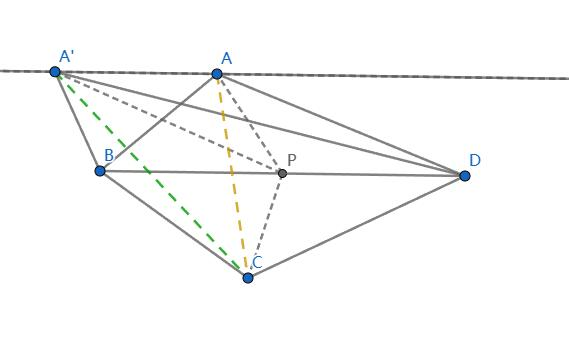
\includegraphics[scale=1]{./2022T7fig.jpg}
8. 三位数中任意两个数字之和都能被第三个数整除, 求这样的三位数的个数\\
 解:\\
case 1 : 该三位数各位数字相等, 显然有 9 个, \\
case 2 : 该三位数各位数字不等, 有: $(1,2,3),(2,4,6),(3,6,9)$, 一共 $3 A_3^3=18$ 个, \\
case 3 : 该三位数有且仅有 2 位数相同, 有: $(1,1,2),(2,2,4),(3,3,6),(4,4,8)$, 一共 $4 C_3^1=12$ 个, 故这样的三位数有 $: 9+18+12=39$ 个.\\\\
二.解答题(12分)\\
请用3种方法证明: $\displaystyle\left(\frac{\alpha+\beta+\gamma}{3}\right)^3 \geq \alpha \cdot \beta \cdot \gamma\left(\alpha, \beta, \gamma \in \mathbb{R}^{+}\right)$.\\
解: \\
$\text{法一:}\\$ 根据基本不等式 $\displaystyle\frac{\alpha+\beta}{2} \geq \sqrt{\alpha \beta}$,
故: $\displaystyle\frac{\alpha+\beta+\gamma+\eta}{4}=\frac{\frac{\alpha+\beta}{2}+\frac{\gamma+\eta}{2}}{2} \geq \sqrt{\sqrt{\alpha \beta} \sqrt{\gamma \eta}}=\sqrt[4]{\alpha \cdot \beta \cdot \gamma \cdot \eta}$,\\
令 $\displaystyle\eta=\frac{\alpha+\beta+\gamma}{3}$, 有: $\displaystyle\frac{\alpha+\beta+\gamma}{3} \geq \sqrt[3]{\alpha \cdot \beta \cdot \gamma}$, 证毕\\
$\text{法二:}\\$ 令 $\alpha=x^3, \beta=y^3, \gamma=z^3$, 则:\\
$\displaystyle
\frac{x^3+y^3+z^3}{3}-x y z\\
=\frac{1}{3}\left(x^3+y^3+z^3-3 x y z\right)\\
=\frac{1}{3}\left\{\left[(x+y)^3-3 x^2 y-3 x y^2\right]+z^3-3 x y z\right\} \\
=\frac{1}{3}\left\{\left[(x+y)^3+z^3\right]-3 x^2 y-3 x y^2-3 x y z\right\}\\
=\frac{1}{6}(x+y+z)\left[(x-y)^2+(y-z)^2+(z-x)^2\right] \geq 0\\
$
证毕\\
 $
\text{法三:}\\ 
\text { 令 } f(x)=\ln x \text {, 则: } f^{\prime}(x)=\frac{1}{x}, f^{\prime \prime}(x)=-\frac{1}{x^2}<0,
$\\
故: $f(x)$ 是上凸函数, 根据琴生不等式, $\displaystyle\ln \frac{\alpha+\beta+\gamma}{3} \geq \frac{1}{3}(\ln \alpha+\ln \beta+\ln \gamma)$, 证毕\\
三.解答题(16分)\\
已知: $f(x)=\beta x-\ln x-1$,\\
(i) : 若 $f(x) \geq 0$ 恒成立, 求 $\beta$ 的最小值;\\
(ii): 求证: $\displaystyle\frac{1}{x e^x}+x+\ln x \geq 1$;\\
(iii): 若 $\alpha\left(e^{-x}+x^2\right) \geq x-x \ln x$ 恒成立, 求 $\alpha$ 的取值范围\\
解: (i): $f(x)$ 的定义域是 $(0,+\infty), f(x) \geq 0 \Rightarrow \beta x-\ln x-1 \geq 0$,
$\Rightarrow \beta \geq \frac{\ln x+1}{x}$,\\
 令 $\displaystyle g(x)=\displaystyle\frac{\ln x+1}{x}, g^{\prime}(x)=-\frac{\ln x}{x^2}$,\\
当 $x \in(0,1)$ 时, $g^{\prime}(x)>0, g(x)$ 单调增, 当 $x \in(1,+\infty)$ 时, $g^{\prime}(x)<0, g(x)$ 单调减\\
 故 $g_{\text {max }}(x)=g(1)=1$, 即: $\beta \geq g_{\text {max }}(x)=1, \beta$ 的最小值为1.\\
证明:(ii): 当 $\beta=1$ 时, 有: $\ln x \leq x-1$,\\
令 $\displaystyle\frac{1}{x e^x}=t$, 则 $:-x-\ln x=\ln t \leq t-1=\frac{1}{x e^x}-1$,
即: $\displaystyle\frac{1}{x e^x}+x+\ln x \geq 1$.\\
解: (iii): $\alpha\left(e^{-x}+x^2\right) \geq x-x \ln x \Rightarrow \alpha\left(\displaystyle\frac{1}{x e^x}+x\right) \geq 1-\ln x$,\\
注意到: $\displaystyle\frac{1}{x e^x}+x>0$, 即: $\displaystyle \alpha \geq \displaystyle\frac{1-\ln x}{\displaystyle\frac{1}{x e^x}+x}$,\\ 由(ii) 知: $\displaystyle\frac{1-\ln x}{\frac{1}{x e^x}+x} \leq 1$,
且 $x e^x=1$ 时, $\displaystyle\frac{1-\ln x}{\displaystyle\frac{1}{x e^x}+x}=1$,\\
 故 $: \alpha \geq 1, \alpha$ 的取值范围是 $[1,+\infty)$. \\
\section*{2021年启明考试数学部分}
\noindent
1.$\displaystyle x,y,z\in\mathbb{Q},\sqrt{3+\sqrt{2}+\sqrt{3}+\sqrt{6}}=\sqrt{x}+\sqrt{y}+\sqrt{z},xyz=.$\\
解:\\
$\sqrt{3+\sqrt{2}+\sqrt{3}+\sqrt{6}}=\sqrt{x}+\sqrt{y}+\sqrt{z}\\
\Rightarrow x+y+z+2(\sqrt{xy}+\sqrt{yz}+\sqrt{xz})=3+\sqrt{2}+\sqrt{3}+\sqrt{6}$
由于$x,y,z\in\mathbb{Q}$,因此不妨设:
$\left\{\begin{array}[l]{c}
	x+y+z=3\\
	2\sqrt{xy}=\sqrt{2}\\
	2\sqrt{yz}=\sqrt{3}\\
	2\sqrt{xz}=\sqrt{6}
\end{array}\right.
$$\Rightarrow\displaystyle
\left\{\begin{array}[l]{c}\displaystyle
	x=1\\
    \displaystyle y=\frac{1}{2}\\
	\displaystyle z=\frac{3}{2}\\
\end{array}\right.$\\
故:$\displaystyle xyz=\frac{3}{4}$\\
2.$\displaystyle f(x)\geq0,f^2(x+1)+f^2(x)=73(x\in\mathbb{R}).\text{当}x\in[0,1)\text{时}$,$f(x)=10-|13x-4|$,$\displaystyle f(\frac{2021}{13})=$\\
解:$f^2(x+1)+f^2(x)=73\Rightarrow f^2(x+2)+f^2(x+1)=73\Rightarrow f^2(x+2)=f^2(x)$\\
$\because f(x)\geq0\therefore f(x+2)=f(x)$\\
$\displaystyle f(\frac{2021}{13})=f(\frac{19}{13})$,又$\displaystyle\because f^2(\frac{19}{13})+f^2(\frac{6}{13})=73$\\
解得:$\displaystyle f(\frac{2021}{13})=3$\\
3.$\displaystyle y=\frac{4\sin\theta\cos\theta+3}{\sin\theta+\cos\theta}(-\frac{\pi}{4}<\theta<\frac{3\pi}{4}),\text{则 }y\text{ 的最小值为}$\\
$\displaystyle y=\frac{2(1+2\sin\theta\cos\theta)+1}{\sin\theta+\cos\theta}=\frac{2(\sin\theta+\cos\theta)^2+1}{\sin\theta+\cos\theta}=2(\sin\theta+\cos\theta)+\frac{1}{\sin\theta+\cos\theta}\geq2\sqrt{2}$\\
当且仅当$\displaystyle2(\sin\theta+\cos\theta)=\frac{1}{\sin\theta+\cos\theta}$,即$\displaystyle\theta=\frac{7\pi}{12}or-\frac{\pi}{12}$取$"="$\\
4.$\displaystyle\{a_n\}\text{是等差数列},\text{且}a_3=-13,a_7=3.S_n=\sum_{i=1}^na_n,\text{则}(S_n)_{min}=$\\
$\left\{\begin{array}[l]{c}\displaystyle
a_1+2d=-13\\
a_1+6d=3\\	
\end{array}\right.
\Rightarrow\left\{\begin{array}[l]{c}\displaystyle
	a_1=-21\\
	d=4\\	
\end{array}\right.$\\
易知$n=6,(S_n)_{\min}=-66$\\
5.$\displaystyle w=\cos\frac\pi5+i\sin\frac\pi5,\text{则以}w,w^3,w^7,w^9\text{ 为解的方程为}.$\\
解:由棣莫弗定理易知:$w^5=-1$,因此以$w,w^3,w^7,w^9$为解的方程等价于以$w,-w^2,w^3,-w^4$为解的方程.\\
易知:$-1,w,-w^2,w^3,-w^4\text{是}(x+1)(x^4-x^3+x^2-x+1)=0$的根.\\
故以$w,w^2,w^3,w^4$为解的方程是$x^4+x^3+x^2+x+1=0$\\
6. A, B是椭圆 $\displaystyle\frac{x^2}{a^2}+\frac{y^2}{b^2}=1(a>b>0)$ 上两点,O是原点,OA$\perp$OB,则$|AB|_{min}=$\\
解:根据题意不妨设 $\displaystyle A\left(r_1 \cos \theta, r_1 \sin \theta\right), B\left[r_2 \cos \left(\theta+\frac{\pi}{2}\right), r_2 \sin \left(\theta+\frac{\pi}{2}\right)\right]$, \\
则
$\displaystyle
B\left(-r_2 \sin \theta, r_2 \cos \theta\right)$, $A B^2=r_1^2+r_2^2,$ $\displaystyle\frac{r_1^2 \cos ^2 \theta}{a^2}+\frac{r_1^2 \sin ^2 \theta}{b^2}=1,$\\$ \displaystyle
r_1^2=\frac{a^2 b^2}{b^2 \cos ^2 \theta+a^2 \sin ^2 \theta},$$\displaystyle \frac{r_2^2 \sin ^2 \theta}{a^2}+\frac{r_2^2 \cos ^2 \theta}{b^2}=1, r_2^2=\frac{a^2 b^2}{b^2 \sin ^2 \theta+a^2 \cos ^2 \theta} .
$
$$
\begin{aligned}
	\text { 故 } r_1^2+r_2^2 & =\frac{a^2 b^2\left(a^2+b^2\right)}{\left(b^2 \cos ^2 \theta+a^2 \sin ^2 \theta\right)\left(b^2 \sin ^2 \theta+a^2 \cos ^2 \theta\right)} \\
	& =\frac{a^2 b^2\left(a^2+b^2\right)}{\left(a^4+b^4\right) \sin ^2 \theta \cdot \cos ^2 \theta+a^2 b^2\left(\sin ^4 \theta+\cos ^4 \theta\right)} \\
	& =\frac{a^2 b^2\left(a^2+b^2\right)}{\left(a^4+b^4\right) \sin ^2 \theta \cdot \cos ^2 \theta+a^2 b^2\left(1-2 \sin ^2 \theta \cdot \cos ^2 \theta\right)} \\
	& =\frac{a^2 b^2\left(a^2+b^2\right)}{\left(a^2-b^2\right)^2 \sin ^2 \theta \cdot \cos ^2 \theta+a^2 b^2}=\frac{4 a^2 b^2\left(a^2+b^2\right)}{\left(a^2-b^2\right)^2 \sin ^2 2 \theta+4 a^2 b^2} \\
	& \geqslant \frac{4 a^2 b^2\left(a^2+b^2\right)}{\left(a^2+b^2\right)^2} .
\end{aligned}
$$
当且仅当 $\displaystyle\theta=k \pi \pm \frac{\pi}{4}(k \in \mathbf{Z})$ 时等号成立.
因此,线段 $A B$ 长的最小值为 $\displaystyle\frac{2 a b \sqrt{a^2+b^2}}{a^2+b^2}$.\\
7.双曲线:$\displaystyle\Gamma\frac{x^2}4-\frac{y^2}5\:=\:1,$过右焦点作一条长度为$4\sqrt{3}$的弦 $AB$,$A,B$位于右支上。将双曲线$\Gamma$绕其右准线旋转90°,则弦 $AB$形成的曲面面积为\\
解:分析易知弦$AB$扫过的面积为一圆台侧面积的$\displaystyle\frac{1}{4}$.
设$A,B$两点到右准线$\displaystyle l:x=\frac{4}{3}$的距离分别为$r_1,r_2$,\\由于双曲线离心率$\displaystyle e=\frac{3}{2}$,故$\displaystyle S=\frac{1}{4}\pi(r_1+r_2)|AB|=\frac{1}{4e}\pi|AB|^2=8\pi$\\
8.$\text{三种方法求}x(x+1)(x+2)(x+3)\text{ 最小值.}$\\
法一:
不妨设 $\displaystyle y = x + \frac{3}{2}$,则 $\displaystyle x = y - \frac{3}{2}$,代入 $x(x+1)(x+2)(x+3)$ 中得到:
$\begin{aligned}
	&x(x+1)(x+2)(x+3)\\
	=& (y-\frac{3}{2})(y-\frac{1}{2})(y+\frac{1}{2})(y+\frac{3}{2}) \\
	=& (y^2 - \frac{9}{4})(y^2 - \frac{1}{4}) \\
	=& y^4 - \frac{5}{2}y^2 + \frac{9}{16}\\
	=&(y^2-\frac{5}{4})^2-1
\end{aligned}
$\\ 
由于 $y^2\geq 0$,所以 $\displaystyle x(x+1)(x+2)(x+3) \geq-1$,等号成立当且仅当 $\displaystyle y^2 = \frac{5}{4}$,即 $\displaystyle x = \frac{\pm\sqrt{5}-3}{2}$\\
法二:
\begin{align*}
	&\frac{d}{dx} [x(x+1)(x+2)(x+3)]\\
	 &= (x+1)(x+2)(x+3) + x(x+2)(x+3) + x(x+1)(x+3) + x(x+1)(x+2) \\
	&= 4x^3 + 18x^2 + 11x + 6\\
	&=(4x+6)(x^2+3x+1)
\end{align*}
令导函数等于 $0$,解得 $\displaystyle x = -\frac{3}{2}$ 或 $\displaystyle x = \frac{\pm\sqrt{5}-3}{2}$带入原函数中可得最小值在$\displaystyle x = \frac{\pm\sqrt{5}-3}{2}$取得,结果为$-1$。\\
法三:\\
$\begin{aligned}
	&x(x+1)(x+2)(x+3)\\
	=&x(x+3)(x+1)(x+2)\\
	=&(x^2+3x)(x^2+3x+2)\\
	=&(x^2+3x+1-1)(x^2+3x+1+1)\\
	=&(x^2+3x+1)^2-1\geq-1(x^2+3x+1=0,\text{即}\displaystyle x = \frac{\pm\sqrt{5}-3}{2}\text{取得})
\end{aligned}$\\
9.已知$\displaystyle0<a<b$,$\displaystyle\text{证}\frac{\ln b-\ln a}{b-a}>\frac{2a}{a^2+b^2}.$\\
证明:原式等价于要证:$\displaystyle\ln\frac{b}{a}>\frac{2a(b-a)}{a^2+b^2}=\frac{2(\frac{b}{a}-1)}{1+(\frac{b}{a})^2}$\\
$\displaystyle t=\frac{b}{a}\in(1,+\infty)$,即证:$(1+t^2)\ln t>2t-2$\\
注意到$\displaystyle\ln t >1-\frac{1}{t}, t\in(1,+\infty)$,即证:$\displaystyle(1+t^2)\ln t>(1+t^2)(1-\frac{1}{t})>2t-2$,\\
即证:$\displaystyle t^2-3t-\frac{1}{t}+3>0$,而此式求导易证
\section*{2019年启明考试数学部分}
\noindent
1.$37,23,19,5.....$以此类推,第五个数为:\\
解:1\\
2.今天星期六,则 $3^{1998}$ 天后是星期几\\
解:注意到$\displaystyle3^{1998}=(27)^{666}=(28-1)^{666}=1+\sum_{k=0}^{665}C_{666}^k(28)^{666-k}(-1)^k=7N+1$\\
故为星期天.\\
3.$\text{若}x\text{满足}x+x^{-1}=-1,\text{求}x^{2019}+x^{-2019}.$\\
$x+x^{-1}=-1\Rightarrow x^2+x+1=0$,则$\displaystyle x=-\frac12\pm\frac{\sqrt{3}}2i=e^{\pm\frac{2\pi}3i}$(欧拉公式).\\
由棣莫弗定理易得$x^{2019}=e^{\pm1046\pi i}=1$\\
故 $x^{2019}+x^{-2019}=2$.\\
4.$\text{求方程}13\sin x=x\text{的根}.$\\
作图: \\
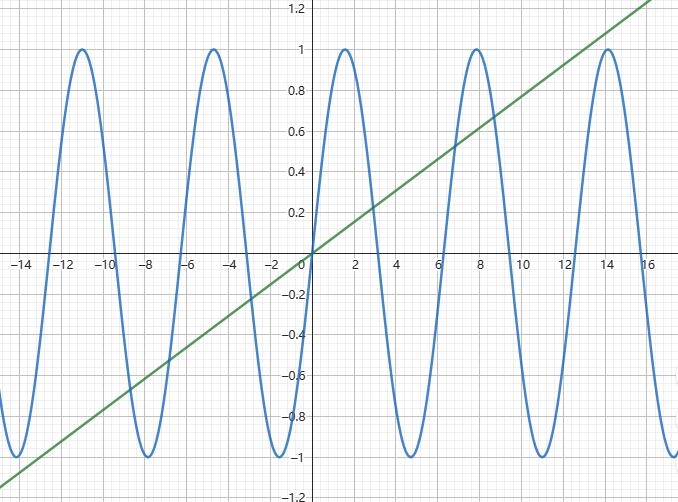
\includegraphics[scale=0.7]{./2019_4.jpg}\\
可以求得的零点为$x=0$,由于此方程为超越方程,其他6个零点为隐零点.\\
5.设整数数列 $a_1,a_2,...a_{10}$ 满足 ${a_{10}=3a_1,a_2+a_8=2a_5.\text{且}a_{i+1}\in\{1+a_i,2+a_i\}}$$(i=1,2,3...9),\text{求这样的数列有多少个}.$\\
不妨设$b_i=a_{i+1}-a_i\in\{1,2\}$,由$a_{10}=3a_1,a_2+a_8=2a_5$,可得:\\
$\begin{cases}
	\displaystyle2a_1=\sum_{i=1}^9b_i\\
	b_7+b_6+b_5=b_4+b_3+b_2
\end{cases}$\\
对于$	b_7+b_6+b_5=b_4+b_3+b_2$,分析易知等式两端 $1,2$的个数相等,因此$b_7,b_6,b_5,b_4,b_3,b_2$总的取法共有:$(C_3^0)^2+(C_3^1)^2+(C_3^2)^2+(C_3^3)^2=20$种\\
注意到$b_7+b_6+b_5+b_4+b_3+b_2$必是偶数,由$\because\displaystyle2a_1=\sum_{i=1}^9b_i$, $2a_1$也为偶数\\
故$b_1+b_8+b_9$必为偶数,取法有4种\\
故满足条件的数列共有$4\times20=80$种\\
6.$\text{求}n^3+100\text{能被}n+10\text{整除的最大整数}.$\\
$\begin{aligned}
	&\frac{n^3+100}{n+10}\\
	=&\frac{n^{3}+1000}{n+10}-\frac{900}{n+10} \\
	=&n^2-10n+100-\frac{900}{n+10}
\end{aligned}$\\
$\Rightarrow n_{max}=890$\\
7.$x,y,z$为非负整数,且 $\left\{\begin{array}{l}x+y+z={10}\quad\text{\ding{172}}\\x+{2}y+{3}z={30}\text{\ding{173}}\end{array}\right.$ ,求$x+5y +3z$的取值范围\\
解:$3\times\text{\ding{172}}-\text{\ding{173}}\Rightarrow2x+y=0$\\
$\because x,y\in\mathbb{N^*}\therefore x=y=0\Rightarrow z=10$\\
故$x+5y +3z=30$\\
8.$\text{若}f(x)=(1-x^2)\left(x^2+ax+b\right)\text{关于}x=-2\text{对称,求}f(x)_{\max}.$\\
解:注意到$x=-1,1$为$f(x)$的零点,又$\because x=-2$为其对称轴,因此可得另两个零点为:$x=-3,x=-5$\\
故$f(x)=(1-x^2)(x+3)(x+5)$\\
$\begin{aligned} 
	\text{注意到:}f(x)&=(1-x)(x+5)(1+x)(x+3)\\
	&=(-x^2-4x+5)(x^2+4x+3)\\
	&\leq(\frac{-x^2-4x+5+x^2+4x+3}{2})^2\\
	&=16(\text{当且仅当}-x^2-4x+5=x^2+4x+3\text{取得})
\end{aligned}$\\
9.$\text{若}\alpha,\beta\text{满足}\left\{\begin{array}{l}x\sin\beta+y\cos\alpha=\sin\alpha\\x\sin\alpha+y\cos\beta=\sin\beta\end{array},\text{求}x^2-y^2.\right.$\\
\\分析:不要被题设吓到,实际上就是解二元一次方程组\\
$\left\{\begin{array}{l}x\sin\beta+y\cos\alpha=\sin\alpha\\x\sin\alpha+y\cos\beta=\sin\beta\end{array}\right.\Rightarrow\left\{\begin{array}{l}\displaystyle x=\frac{\sin\beta\cos\alpha-\sin\alpha\cos\beta}{\sin\alpha\cos\alpha-\sin\beta\cos\beta}\\\displaystyle y=\frac{\sin^2\alpha-\sin^2\beta}{\sin\alpha\cos\alpha-\sin\beta\cos\beta}\end{array}\right.$\\
$\begin{aligned}
	x&=\frac{\sin\beta\cos\alpha-\sin\alpha\cos\beta}{\sin\alpha\cos\alpha-\sin\beta\cos\beta}=\frac{2\sin(\alpha-\beta)}{\sin2\alpha-\sin2\beta}\\
	&=\frac{2\sin(\alpha-\beta)}{2\cos(\alpha+\beta)\sin(\alpha-\beta)}=-\sec(\alpha+\beta)
\end{aligned}
$\\
$\begin{aligned}
	y&=\frac{\sin^2\alpha-\sin^2\beta}{\sin\alpha\cos\alpha-\sin\beta\cos\beta}=\frac{\cos2\beta-\cos2\alpha}{\sin2\alpha-\sin2\beta}\\
	&=\frac{\sin(\alpha+\beta)\sin(\alpha-\beta)}{\sin(\alpha-\beta)\cos(\alpha+\beta)}=\tan(\alpha+\beta)
\end{aligned}
$\\
故$x^2-y^2=1$\\
10.$A(3,2)$是平面上一点,$F$是抛物线:$y^2=2x$上的一点,抛物线上一点$M$,则$|MF|+|MA|$取最小值的时$M$的坐标\\
解:很简单的高中题.由题意得$\displaystyle F(\frac12,0)$,准线方程为$\displaystyle x=-\frac12$,设点$M$到准线的距离为$d=|PM|$.则由抛物线的定义得$|MA|+|MF|=|MA|+|PM|$
故当$P,A,M$三点共线时,$|MF|+|MA|$取得最小值为 $\displaystyle|AP|=3-(-\frac{1}{2})=\frac{7}{2}.$
把$y = 2$代入抛物线$y^2 = 2x$得$x = 2$,故点M的坐标是$(2,2)$\\
附个图:\\
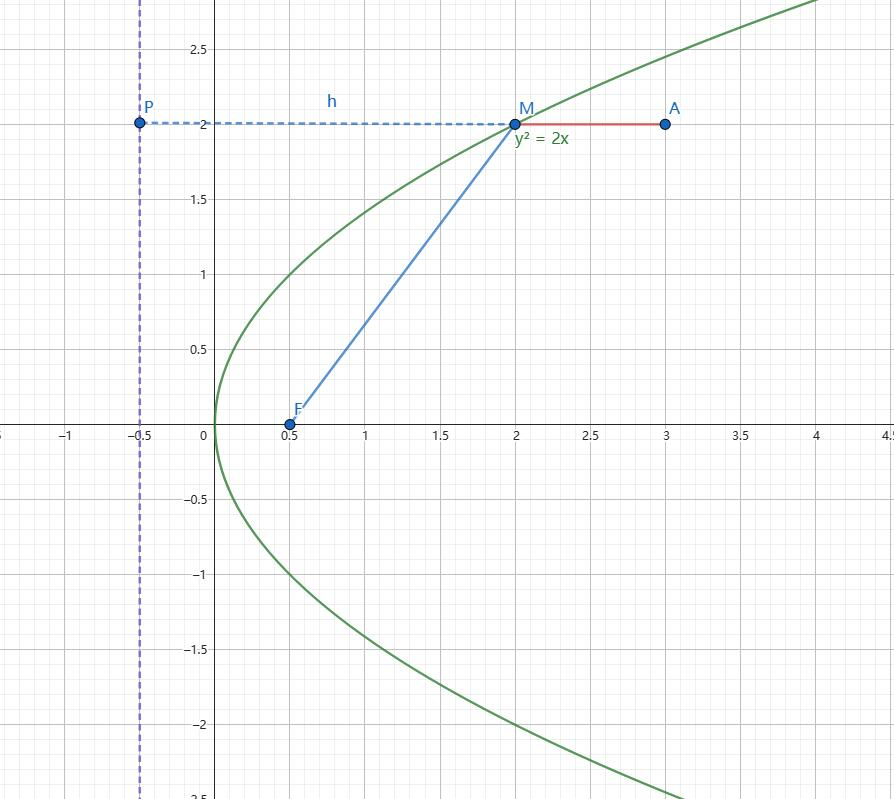
\includegraphics[scale=0.3]{./2019_10.jpg}\\
11.$\forall x,y \in\mathbb{R},$函数$f(z)$满足$2f(x)f(y)= f(x+y)+f(x-y)$且$f(x)\neq0$,证明:$f^2(x)+f^2(y)=f(x+y)f(x-y)+1$\\
令$x=y=0\Rightarrow f(0)=1$\\
$2f(x)f(y)= f(x+y)+f(x-y)\Rightarrow2f(x+y)f(x-y)= f(2x)+f(2y)(\mathbf{*})$\\
令$x=y\Rightarrow2f^2(x)=f(2x)+f(0)=f(2x)+1$,同理$2f^2(y)=f(2y)+1$\\带入$(\mathbf{*})$中得:$f^2(x)+f^2(y)=f(x+y)f(x-y)+1$\\
12.数列$\{a_n\}$满足$\displaystyle a_1=3,a_{n+1}\leq\frac12(a_n+a_{n+2}),\text{且}a_{505}=2019.\text{求}\mathrm{max}a_5$.\\
分析:一个自然的想法是所有的等号均能取得时$a_3$取得最大值,此时$\{a_n\}$为$d=4$的等差数列,解得$a_5=19$\\
令$\displaystyle b_n=a_{n+1}-a_n$,$\displaystyle a_{n+1}\leq\frac12(a_n+a_{n+2})\Rightarrow b_{n}\leq b_{n+1}$\\
$\therefore a_5=a_1+b_1+b_2+b_3+b_4$\\
$\displaystyle a_{505}-a_1=\sum_{i=1}^{504}b_i\geq126(b_1+b_2+b_3+b_4)\Rightarrow b_1+b_2+b_3+b_4\leq16$\\
$\therefore a_3=a_1+b_1+b_2+b_3+b_4\leq19,\text{当}\{a_n\}\text{为等差数列取}\text{“=”}$\\
13.$f(a)$是$\mathbb{R}$上的偶函数,函数图像关于$x=1$对称。对任意的 $\displaystyle x,y\in\left[{0},\frac12\right]$$\text{有}f(x+y)=f(x)f(y),\text{且}f(1)=\beta>0.$\\
(1)$\displaystyle\text{求}f{\left(\frac12\right)},f{\left(\frac14\right)}\text{的值}.$\\
(2)证明:$f(x)$是周期函数\\
(3)$\displaystyle\text{记}\beta(n)=f\left(2n+\frac1{2n}\right),\text{求}\lim_{n\to\infty}\ln\beta(n).$\\
解:(1)易得:$\displaystyle f(\frac{1}{2})=\beta^\frac{1}{2},f(\frac{1}{4})=\beta^\frac{1}{4}$\\
证明:(2)事实上,由双镜原理周期为2是显然的\\
$f(2+x)=f(-x)=f(x)\Rightarrow f(x)\text{是}T=2\text{的周期函数}$\\
解:(3)$\displaystyle\beta(n)=f\left(2n+\frac1{2n}\right)=f(\frac{1}{2n})$\\
注意到:$\displaystyle f(\frac{1}{2})=f(n\times\frac{1}{2n})=f^n(\frac{1}{2n})\Rightarrow f(\frac{1}{2n})=\beta^{\frac{1}{2n}}$\\
$\displaystyle\therefore \beta(n)=\ln f(\frac{1}{2n})=\frac{\beta}{2n}\rightarrow0(n\to\infty)$
\section*{2015年启明考试数学部分}
\noindent
一、填空题\\
1.对抛物线 $y^2=2 \sqrt{2} x$, 若设其焦点为 $F, y$ 轴正半轴上一点为 $N$. 若准线上存在唯一的点 $P$ 使得 $\angle N P F=90^{\circ}$, 则 $N$ 点的纵坐标为\\
分析:实际上就是以$NF$为直径的圆与准线相切,求此时 $N$点坐标,图如下:\\
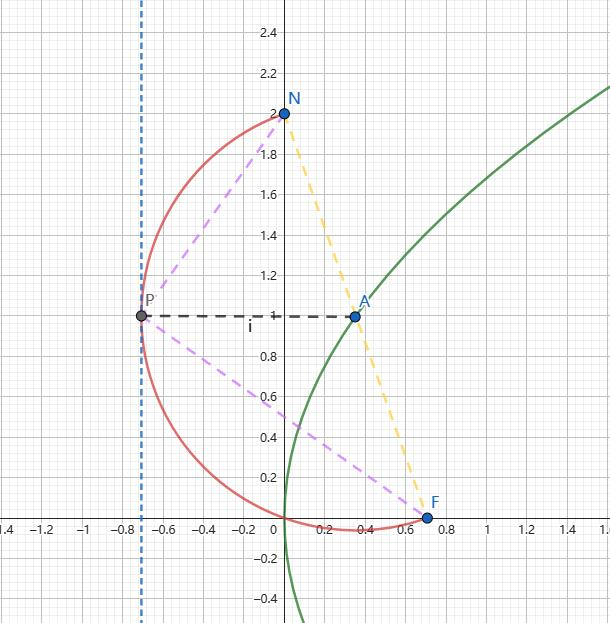
\includegraphics[scale=0.5]{./2015_1.jpg}\\
$|AP|=|AN|=|AF|,AP\perp l: x= \frac{\sqrt{2}}{2}\Rightarrow A$在抛物线上\\
设$\displaystyle N(0,a)\Rightarrow A(\frac{\sqrt{2}}{4},\frac{a}{2})$带入抛物线方程,解得$a=2$\\
2. $\displaystyle\frac{1}{\sqrt{1}+\sqrt{2}}+\frac{1}{\sqrt{2}+\sqrt{3}}+\cdots+\frac{1}{\sqrt{255}+\sqrt{256}}=$\\
解:设$\displaystyle b_n=\frac{1}{\sqrt{n+1}+\sqrt{n}}=\sqrt{n+1}-\sqrt{n}$\\
$\displaystyle\frac{1}{\sqrt{1}+\sqrt{2}}+\frac{1}{\sqrt{2}+\sqrt{3}}+\cdots+\frac{1}{\sqrt{255}+\sqrt{256}}=\sum_{i=1}^{255}b_i=\sqrt{256}-1=15$\\
3.若已知 $\displaystyle\lim _{n \rightarrow\infty}\left(\sum_{i=1}^n \frac{1}{i}-\ln n\right)$ 存在, 则 $\displaystyle\sum_{i=0}^{\infty} \frac{(-1)^{i}}{i+1}=$\\
这道题超纲太多了,涉及到级数知识,仅展示做法\\
法一:\\
设$\displaystyle H(n)=\sum_{k=1}^{n}\frac{1}{k}\Rightarrow H(n)=\gamma+\ln n+o(1)$\\
考虑部分和:
$\displaystyle S_{2n}=\sum_{i=1}^{2n}{\frac{(-1)^{i-1}}{i}}=\sum_{i=1}^{n}\frac{1}{2i-1}-\sum_{i=1}^{n}\frac{1}{2i}=\sum_{i=1}^{2n}\frac{1}{i}-\sum_{i=1}^{n}\frac{1}{i}=H(2n)-H(n)=\ln2+o(1)\rightarrow \ln2(n\rightarrow\infty)$\\
$\displaystyle S_{2n+1}=S_{2n}+\frac{1}{2n+1}\rightarrow\ln2(n\rightarrow\infty)$\\
综上:$\displaystyle\sum_{i=0}^{\infty} \frac{(-1)^{i}}{i+1}=\ln2$\\
法二:
注意到:$\displaystyle\ln(1+x)=\sum^\infty_{n=1}\frac{(-1)^{n-1}}{n}x^n\Rightarrow\ln2=\sum^\infty_{n=1}\frac{(-1)^{n-1}}{n}$\\
4.在边长为 1 的正方形中 (含边界) 取9 个点, 其中必有 3 个点, 它们构成的三角形面积不超过\\
解:在边长为 $\text{1}$ 的正方形内任取3个点,则这3点组成的三角形的面积不超过$\displaystyle\frac{1}{2}$。若我们在一个边长为$\displaystyle\frac{1}{2}$的正方形内任取3点,那么这3点所
组成的三角形的最大面积就是这个正方形的面积的一半,即不超过$\displaystyle\frac{1}{8}$。那么我们将一个边长为 $\text{1}$ 的正方形分为4个相同的边长为 $\displaystyle\frac{1}{2}$的小正方形,任取9个点放到正方形中,必有3个点落在同一个小正方形内。\\
由上面的分析得知,这3个点所组成的三角形面积不超过$\displaystyle\frac{1}{8}$\\
5.某人打靶打中 8 环、 9 环、 10 环的概率分别为 $0.15,0.25,0.2$, 现他开三枪, 不少于 28 环的概率为\\
解:
case 1:成绩为28环,有以下情况:$\{9,9,10\},\{8,10,10\}$\\
case 2:成绩为29环,有以下情况:$\{9,10,10\}$\\
case 3:成绩为30环,有以下情况:$\{10,10,10\}$\\
$p=\mathbf{C}_3^20.25^2\cdot0.2+\mathbf{C}_3^20.2^2\cdot0.15+\mathbf{C}_3^20.2^2\cdot0.25+0.2^3=0.0935$\\
二、解答题\\
6.若对任意实数 $x, y$, 有 $f\left((x-y)^2\right)=(f(x))^2-2 x  f(y)+y^2$, 求 $f(x)$.\\
解:令$x=y\Rightarrow f(0)=f^2(x)-2xf(x)+x^2=(f(x)-x)^2$\\
再令$x=0\Rightarrow f(0)=0or1\\\Rightarrow f(x)=x\quad or\quad f(x)=x+1$\\
7.求所有 $a, b$, 使 $\displaystyle\left|\sqrt{1-x^2}-a x-b\right| \leqslant \frac{\sqrt{2}-1}{2}$ 成立, 其中 $x \in[0,1]$.\\
不妨设$x=\sin\theta,\theta\in[0,\frac{\pi}{2}]$\\
$\begin{aligned}
	&\left|\sqrt{1-x^2}-a x-b\right|\\
	=&|\cos\theta-a\sin\theta-b|\\								   
	=&|\sqrt{a^2+1}\sin(\theta+\phi)-b|\leq\frac{\sqrt{2}-1}{2}(\tan\phi=-\frac{1}{a})
\end{aligned}$\\
$\Rightarrow \frac{1-\sqrt{2}}{2}+b\leq\sqrt{a^2+1}\sin(\theta+\phi)\leq\frac{\sqrt{2}-1}{2}+b\quad(*)$\\
$f(\theta):=\sqrt{a^2+1}\sin(\theta+\phi)$\\
case 1:$a\geq0$\\
$\displaystyle[f(\theta)]_{max}=f(\frac{\pi}{2})=\sqrt a,[f(\theta)]_{min}=f(0)=-1$\\
注意到此时值域区间长度$l=a+1>\sqrt{2}-1,(*)$必不能恒成立,此种情况舍去\\
case 2:$a<0$\\
$\displaystyle[f(\theta)]_{max}=f(\frac{\pi}{2}-\phi)=\sqrt{a^2+1},[f(\theta)]_{min}=\min\{f(\frac{\pi}{2}),f(0)\}=\min\{-a,1\}$\\
if $\displaystyle a\leq-1,\Rightarrow[f(\theta)]_{min}=1$,区间长度$l=\sqrt{a^2+1}-1\leq\sqrt{2}-1\Rightarrow a\in[-1,1]\Rightarrow a=-1$\\
$\displaystyle [f(\theta)]_{min}=1=\frac{1-\sqrt{2}}{2}+b\Rightarrow b=\frac{\sqrt{2}+1}{2}$\\
if $a>-1,\Rightarrow[f(\theta)]_{min}=-a$,此时区间长度$l=\sqrt{a^2+1}+a>\sqrt{2}-1,(*)$必不能恒成立,此种情况舍去\\
综上所述:$\displaystyle a=-1,b=\frac{\sqrt{2}+1}{2}$\\
8.若复数 $z$ 满足 $|z|=1$, 求 $\left|z^3-z+2\right|^2$ 的最小值.\\
解:\\
法一:\\
设 $z=\cos\theta+i\sin\theta,\text{得}z^{3}-z+2=\cos3\theta-\cos\theta+2+i(\sin3\theta-\sin\theta)$
$\\
\begin{aligned}
	\mid z^{3}-z+2\mid^{2}
	&=\left(\cos3\theta-\cos\theta+2\right)^{2}+\left(\sin3\theta-\sin\theta\right)^{2}\\
	&=6-2\left(\cos3\theta\cos\theta+\sin3\theta\sin\theta\right)+4\cos3\theta-4\cos\theta\\
	&=6-2\cos2\theta+4\cos3\theta-4\cos\theta\\
	&=4\left(4\cos^{3}\theta-\cos^{2}\theta-4\cos\theta+2\right)
\end{aligned}\\
$
求导易得当$\cos\theta=\frac{2}{3}\text{时}\:,\left(\:|z^{3}-z+2\:|^{2}\right)_{\mathrm{min}}=\frac{8}{27}.$\\
法二:\\
$\begin{aligned}
	& \left|z^3-z+2\right|^2=\left|z^3-z+2 z \bar{z}\right|^2=\left|z\left(z^2-1+2 \bar{z}\right)\right|^2=\left|z^2-1+2 \bar{z}\right|^2 \\
	& =\left(z^2-1+2 \bar{z}\right)\left(\bar{z^2}-1+2 z\right)=4-2(\mathrm{z}+\bar{z})-\left(z^2+\bar{z}^2\right)+2\left(z^3+\bar{z}^3\right) \\
	& =4-2(z+\bar{z})-\left[(z+\bar{z})^2-2\right]+2(z+\bar{z})\left[(z+\bar{z})^2-3\right] \\
	&\xlongequal{\text { let }, z+\bar{z}=x \in[-2,2]}2 x^3-x^2-8 x+6 \text {(用导数易求最值)}
\end{aligned}$
\\
9.已知三次方程 $x^3+a x^2+b x+c=0$ 有三个实根.\\
(1) 若三个实根为 $x_1, x_2, x_3$, 且 $x_1 \leqslant x_2 \leqslant x_3, a, b$ 为常数, 求 $c$ 变化时 $x_3-x_1$ 的取值范围;\\
(2) 若三个实根为 $a, b, c$, 求 $a, b, c$.\\
解:这题有些麻烦,如果缺少一元三次方程的相关概念建议下去了解一下再来看这道题\\
(1) 设三次方程 $x^3+a x^2+b x+c=0$ 的三个实根分别为 $x_1, x_2, x_3\left(x_1 \leqslant x_2 \leqslant x_3\right)$
由韦达定理, 可得 $x_1+x_2+x_3=-a, x_1 x_2+x_2 x_3+x_3 x_1=b$, 注意到
$$
	\frac{1}{2}[2(\frac{x_3-x_1}{2})^2+\left(x_3-x_1\right)^2]\leq a^2-3 b=\frac{1}{2}\left[\left(x_1-x_2\right)^2+\left(x_2-x_3\right)^2+\left(x_3-x_1\right)^2\right]\leq [\left(x_3-x_1\right)^2] 
$$
$$
	\Rightarrow\sqrt{a^2-3 b} \leqslant x_3-x_1 \leqslant 2 \sqrt{\frac{a^2-3 b}{3}}
$$
当且仅当 $x_1=x_2$ 或 $x_2=x_3$ 时取到左端"=", 当且仅当 $x_1+x_3=2 x_2$ 时取到右端"=". \\
综上所述:$x_3-x_1$ 的取值范围是 $\displaystyle\left[\sqrt{a^2-3 b} \leqslant w \leqslant 2 \sqrt{\frac{1}{3} a^2-b}\right]$.\\
(2) 易知$x^3+a x^2+b x+c=(x-a)(x-b)(x-c)$, 由韦达定理得
$$
\left\{\begin{array}{l}
	a+b+c=-a \\
	a b+b c+c a=b \\
	a b c=-c
\end{array}\right.
$$
$$\Rightarrow c=0 \text{ or } a b=-1$$.\\
if $c=0$, $\left\{\begin{array}{l}b=-2 a \\ a b=b\end{array}\right.$,  $\Rightarrow\left\{\begin{array}{l}a=0 \\ b=0\end{array}\right.$ or $\left\{\begin{array}{l}a=1 \\ b=-2\end{array}\right.$.\\
if $a b=-1$ 时, $\left\{\begin{array}{l}c=-2 a-b \\ -1+(a+b) c=b\end{array}\right.$, 带入原方程,得:
$$
	b^4+b^3-2 b^2+2=0 
$$
$$\Rightarrow 	b+1=0 \text { or } b^3-2 b+2=0$$
if  $b+1=0$, $\Rightarrow\left\{\begin{array}{l}
	a=1 \\
	c=-1
\end{array}\right.$ \\
if $b^3-2 b+2=0$ ,\\ 由一元三次方程的求根公式得 $\displaystyle b=\sqrt[3]{\sqrt{\frac{19}{27}}-1}-\sqrt[3]{\sqrt{\frac{19}{27}}+1}\Rightarrow\left\{\begin{array}{l}
	\displaystyle a=-\frac{1}{b} \\
	\displaystyle c=\frac{2}{2}-b
\end{array}\right.$ \\
综上$(a, b, c)$ 的值为 $(0,0,0),(1,-2,0),(1,-1,-1)$ , $\displaystyle\left(-\frac{1}{k}, k, \frac{2}{k}-k\right)$ (其中 $\displaystyle k=\sqrt[3]{\sqrt{\frac{19}{27}}-1}-\sqrt[3]{\sqrt{\frac{19}{27}}+1}$).\\

\section*{2014年启明考试数学部分}
\noindent
一、填空题 (本题共 5 小题, 每小题8分, 共40分)\\
1.设 $\displaystyle f(x)=\frac{x}{\sqrt{1+x^2}}$, 则 $n$ 重复合函数 $f_n(x)=f(f(\cdots f(x) \cdots))=$\\
解:$\displaystyle f(x)=\frac x{\sqrt{1+x^2}}$计算得 $\displaystyle f_2(x)=\frac x{\sqrt{1+2x^2}},$
$\displaystyle f_3(x)=\frac x{\sqrt{1+3x^2}}$\\
由此猜想:$f(x)$经过n次复合后结果是 $\displaystyle\frac x{\sqrt{1+nx^2}}$,下面用数学归纳法证明:\\
当 $n=1$ 时,显然成立\\
当 $n=k(k{\in}N+)$ 时,$\displaystyle f_k(x)=\frac x{\sqrt{1+kx^2}}$成立.\\
当 $n=k+1$ 时,$f_{k+1}$为 $f(x)$ 和 $f_{k}(x)$ 的复合函数\\
经计算得 $\displaystyle f_{k+1}=\frac{x}{\sqrt{1+(k+1)x^2}}$ 与假设相符,
故假设成立\\
故:$\displaystyle f_n(x)=\frac x{\sqrt{1+nx^2}}$\\
2.设多项式 $p(x)$ 满足 $p\left(x^2+1\right)=(p(x))^2+1$ 和 $p(0)=0$, 则 $p(x)=$\\
答案很明显$p(x)=x$,证明如下:
注意到$p(1)=p(0)^2+1=1,p(2)=p(1)^2+1=2,p(5)=p(2)^2+1=5,...\Rightarrow p(x)=x$有无穷多解\\
又$\because p(x)$为多项式函数(设为$n$次),则$p(x)-x$也为多项式函数\\
但由代数基本定理$p(x)-x=0$最多有$n$个根$\Rightarrow p(x)-x\equiv0\Rightarrow p(x)=x$\\
3.设 $\displaystyle S_n=\sum_{k=1}^n \frac{6^k}{\left(3^{k+1}-2^{k+1}\right)\left(3^k-2^k\right)}$, 则极限 $\displaystyle\lim _{n \rightarrow \infty} S_n=$\\
注意到:\\
$\begin{aligned}
	\displaystyle S_n&=\sum_{k=1}^n \frac{6^k}{\left(3^{k+1}-2^{k+1}\right)\left(3^k-2^k\right)}\\
	&=\sum_{k=1}^n\frac{2^k}{3^{k}-2^{k}}-\frac{2^{k+1}}{3^{k+1}-2^{k+1}}\\
	&=2-\frac{2^{n+1}}{3^{n+1}-2^{n+1}}\rightarrow2(n\to\infty)
\end{aligned}$\\
4.对 $x>0$, 函数 $\displaystyle f(x)=\frac{\left(x+\displaystyle\frac{1}{x}\right)^6-\left(x^6+\displaystyle\frac{1}{x^6}\right)-2}{\left(x+\displaystyle\frac{1}{x}\right)^3+\left(x^3+\displaystyle\frac{1}{x^3}\right)}$ 的最小值为\\
注意到:\\
$\begin{aligned}\displaystyle
	f(x)&=\frac{(x+\displaystyle\frac{1}{x})^6-(x^3+\displaystyle\frac{1}{x^3})^2}{(x+\displaystyle\frac{1}{x})((x+\displaystyle\frac{1}{x})^2+x^2+\displaystyle\frac{1}{x^2}-1)}\\
	&=\frac{(x+\displaystyle\frac{1}{x})^2((x+\displaystyle\frac{1}{x})^4-(x^2+\displaystyle\frac{1}{x^2}-1)^2)}{(x+\displaystyle\frac{1}{x})((x+\displaystyle\frac{1}{x})^2+x^2+\displaystyle\frac{1}{x^2}-1)}\\
	&=\frac{(x+\displaystyle\frac{1}{x})^2((x+\displaystyle\frac{1}{x})^2-(x^2+\displaystyle\frac{1}{x^2}-1))((x+\displaystyle\frac{1}{x})^2+(x^2+\displaystyle\frac{1}{x^2}-1))}{(x+\displaystyle\frac{1}{x})((x+\displaystyle\frac{1}{x})^2+x^2+\displaystyle\frac{1}{x^2}-1)}\\
	&=3(x+\frac{1}{x})\geq6(\text{当且仅当}x=1\text{取得“=”})
\end{aligned}$\\
5.假设 20 名学生中的每一名学生可从提供的六门课程中选学一门至六门, 也可以一门都不 选. 试判断下列命题是否正确: 存在 5 名学生和两门课程, 使得这 5 名学生都选了这两门课, 或者都没选, 选填“正确”或“否”\\
解:答案是否定的.不一定会出现这5个学生.假设20个学生都选三门课,而且选法都不完全一样,因为$\displaystyle20 =\left(^6_3\right)$,所以这是可能的.那么对任何两门课程,恰有4个学生选(他们选的第3门课都不同,4 = 6 - 2门课程中的一门).所以任何两门课程没有5个学生同时选.同样地,对任何两门课程,恰有4个学生没有选取这两门课,而没有5名学生同时不选两门课。\\
二、(本题共14分)\\
1.若 $a$ 为正整数而 $\sqrt{a}$ 不为整数, 证明: $\sqrt{a}$ 为无理数.\\
证明:反证法,设 $\displaystyle\sqrt{a}\in\mathbb{Q}$,从而可进一步设$\sqrt{a}=\frac{p}{q}\quad(p,q\in\mathbb{N^*},(p,q)=1)$
$\Rightarrow p^2=aq^2$
$\because a$不是完全平方数$\therefore \exists m\in\mathcal{P},s.t\quad a\mod m=0,a\mod m^2\neq0$\\
$p^2=aq^2\Rightarrow p^2\mod m =0\Rightarrow p\mod m =0\Rightarrow p^2\mod m^2=0\\\Rightarrow aq^2\mod m^2=0\Rightarrow q^2\mod m=0\Rightarrow q\mod m=0$\\
$\therefore q\mod m=0,p\mod m =0$与 $(p,q)=1$矛盾,故$\sqrt{a}$ 为无理数\\
2.试证:除 $\{0,0,0\}$ 外, 没有其他整数 $m, n, p$ 使得
$$
m+n \sqrt{2}+p \sqrt{3}=0 .
$$
证明:\\
反证法.假设存在整数 $m, n, p$,使得 $m + n\sqrt{2} + p\sqrt{3} = 0$\\
首先考虑含有 $0$的情况,这种情况显然是存在矛盾的,不多赘述\\
下面考虑$m, n, p$全部不为$0$的情况:\\
注意到$n\sqrt{2}$ 和 $p\sqrt{3}$ 也是无理数
对于$m + n\sqrt{2} + p\sqrt{3} = 0$,易得:
$$m = -n\sqrt{2} - p\sqrt{3}$$
$$\Leftrightarrow m^2 = (n\sqrt{2} + p\sqrt{3})^2$$
$$\Leftrightarrow m^2 = 2n^2 + 3p^2 + 2\sqrt{6}np$$
$\because m\in\mathbb{Z}\therefore m^2\in\mathbb{Z}\Rightarrow 2n^2 + 3p^2 + 2\sqrt{6}np\in\mathbb{Z}$\\
但$2\sqrt{6}np$ 是一个无理数。因此,$2n^2 + 3p^2 + 2\sqrt{6}np$ 必是一个无理数。
矛盾,假设不成立。
综上所述,除了 $\{0, 0, 0\}$ 外,不存在其他整数 $m, n, p$ 使得 $m + n\sqrt{2} + p\sqrt{3} = 0$.\\
三、(本题共16分) 设 $a, b, c$ 为三角形三边之长, $\displaystyle p=\frac{a+b+c}{2}, r$ 为内切圆半径, 证明:
$$
\frac{1}{(p-a)^2}+\frac{1}{(p-b)^2}+\frac{1}{(p-c)^2} \geqslant \frac{1}{r^2}
$$
证明: 设三角形的面积为 $S$, 则 $S=p r$, $S=\sqrt{p(p-a)(p-b)(p-c)}$,\\
 $\Rightarrow p^2 r^2=p(p-a)(p-b)(p-c)$.
\\设 $\displaystyle x=\frac{1}{p-a}, y=\frac{1}{p-b}, z=\frac{1}{p-c}$,则有:
$$
\frac{1}{r^2}=p x y z=x y z\left(\frac{1}{x}+\frac{1}{y}+\frac{1}{z}\right)=x y+y z+z x$$
$$
\Leftrightarrow x^2+y^2+z^2 \geqslant x y+y z+z x   
$$
而上式是显然易证的.\\
四、(本题共 12 分) 证明: 设 $m$ 是任一正整数, 则 $\displaystyle \displaystyle a_m=\frac{1}{2}+\frac{1}{3}+\frac{1}{4}+\frac{1}{5}+\cdots+\frac{1}{2^m}$ 不是整 数.\\
证明: 当 $m=1$ 时, $\displaystyle a_1=\frac{1}{2}$, 显然不是整 数, 结论成立.
下面证明, 当 $m \geqslant 2$ 时,
$\displaystyle a_m=\frac{1}{2}+\frac{1}{3}+\frac{1}{4}+\ldots+\frac{1}{2^m}$ 也不可能是 整数.
设 $\displaystyle S=\frac{1}{2}+\frac{1}{3}+\frac{1}{4}+\ldots+\frac{1}{2^m}$, 令 $M=2^m$ ,在 $S$ 两边同时乘以 $M$ 得:
$$
M S=\frac{M}{2}+\frac{M}{3}+\frac{M}{4}+\ldots+1\quad(*)
$$
等式右边的每一项 $\displaystyle\frac{M}{k}\left(k=1,2,3, \ldots, 2^m\right)$
要么是整数, 要么是一个分母为奇数的不可 约分数,
再来考察那些分母为奇数的不可约分数的项.
因为 $m \geqslant 2$, 故在所有的分母当中 (都是奇
数) 必定存在一个最大的奇素数,
设它为 $p$, 这样在分母中去掉 $p$, 设余下的奇数 的最小公倍数为 $N$,
在$(*)$再同时乘以 $N$, 得到
$$
\begin{aligned}
	& M N S=\frac{M N}{2}+\frac{M N}{3}+\frac{M N}{4}+\ldots +N
\end{aligned}
$$
等式右边的每一项$\displaystyle\frac{M N}{k}(k=1,2,3, \ldots, 2^m,k\neq p)$, 仅当$k=p$ 时, $\displaystyle\frac{M N}{k}$不是整数, 其他的项都是整 数.\\
所以等式右边最后得到的不是整数, 因此, 等 式左边的 $M N S$ 也不是整数,
显然, 若 $S$ 是整数, 那么就与 $M N S$ 不是整数 相矛盾!
所以 $a_m$ 不可能是整数. 证毕.\\
五、(本题共18分)下图是2013年恒大足球倶乐部策划的主场与首尔 FC足球队的亚冠决赛 海报, 左边是恒大队, 右边是首尔队, 该海报的寓意是什么? 要求简单推导海报中两个数学 式子的结果. 一个数学式子是 $\sqrt{1+2 \sqrt{1+3 \sqrt{1+4 \sqrt{1+\cdots}}}}$ (拉马努金式子), 另一个是 $\mathrm{e}^{\pi \mathrm{i}}+1$ (已知欧拉公式 $\mathrm{e}^{\pi \mathrm{i}}=\cos \alpha+\mathrm{i} \sin \alpha$ ).\\
解:注意到拉马努金恒等式:$n=\sqrt{1+(n-1)(n+1)}$, 因此: \\
$\begin{aligned}
   3&=\sqrt{1+2\cdot4}  \\
	&=\sqrt{1+2\sqrt{1+3\cdot5}} \\
	&=\sqrt{1+2\sqrt{1+3\sqrt{1+4\cdot6}}}. \\
	&=\ldots 
\end{aligned}$\\
注意到$e^{i\pi}+1=0$,故结果为:$3:0$\\

\includegraphics[scale=0.9]{./2014_l.jpg}\\\\\\
写在最后:

欢迎大家加入2023级学数华科志愿辅导群(855590575),交流数学问题!\\
如果参考答案有些许纰漏欢迎大家指出
\end{document}	
